\documentclass[journal]{IEEEtran}
\usepackage{graphicx}
\usepackage[scriptsize]{caption}
\renewcommand{\arraystretch}{1.1}

\begin{document}

\newcommand{\labtitlegen}{
    \twocolumn[{
    \begin{center}
        \LARGE\labtitle \\ \bigskip \large\name \\ \bigskip
        \labsection \\ 
        \textbf{TA} \\ \taname \\% \bigskip \textbf{Lab Partners} \\
%        \partnername
    \end{center}
    }]
}

%% Change these variables
\newcommand{\labtitle}{Experiment 4: Properties of Sound Waves}
\newcommand{\name}{604-296-523}
\newcommand{\labsection}{Section 2, Wednesday 8AM}
\newcommand{\labdate}{February 18, 2015}
\newcommand{\taname}{Elwin Martin}
\newcommand{\partnername}{Kari Kawashima}


%% This creates your lab cover page.
\labtitlegen

\newcommand{\mval}[3]{$#1 \pm #2 #3$}

\section{Introduction}

Moving a source of a sinusoidal sound wave produces a phase shift at every
point in space relative to the initial signal. Comparing the signal recorded by
a stationary microphone and the signal fed to the sound source shows this phase
shift. This will be used to find the wavelength of sound at various frequencies
- a full phase shift of $2 \pi$ corresponds to the microphone moving through an
entire wavelength.

Sound waves from multiple sources also interfere, and when two waves have the
same frequency but at different locations - for instance, an emitter and a
reflective surface - they form a standing wave. A microphone moving through
this standing wave will observe peaks and troughs in the sound amplitude. This
fact will also be used to measure the wavelength and the corresponding speed of
sound at a single frequency.

\section{Results}

Initially, a microphone was set up on a ruled track, with a sound emitter at
one end of the track. The emitter was connected to a signal generator creating
a pure wine wave. Both the microphone and the signal generator were connected to
an oscilloscope, in such a way that the phase shift of the two channels could be
compared.

The frequency was varied from approximately 3 to 14 kHz, and three measurements
were taken at every frequency - the distance when the waves were initially in
phase, the distance when they are out of phase by half a cycle, and the
distance when they are again in phase. This corresponds to two half-wavelength
displacements, and allows measurement of the entire wavelength.

The data collected here is shown in Figure~\ref{fig:dispersion}, with the wave
number for each frequency being calculated from the measured wavelength.

\begin{figure}[ht!]
\centering
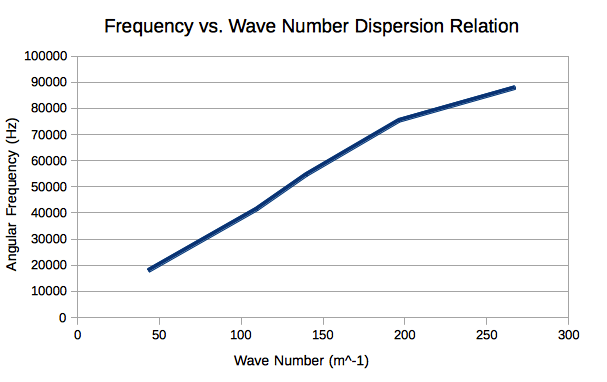
\includegraphics[width=80mm]{dispersion.png}
\caption{Graph of frequency as a function of the wave number ($2 \pi / \lambda$).}
\label{fig:dispersion}
\end{figure}

A sound reflective surface - a sheet of metal - was then placed to the left of
the sound emitter, such that the emitter was between the surface and the
microphone. This allows the microphone to measure the interference of the
emitted and reflected sound waves.

To create a variable phase difference between these sound waves, it is
necessary to move the surface. To collect measurements at close and precisely
measured intervals, the surface was placed on wheels, one of which was a
potentiometer connected to a voltage splitter. To calibrate this device, 2V
were applied to the voltage splitter, and two measurements of the voltage were
taken when moving the surface $20 \pm 0.5$ cm.  There was a voltage drop of
0.1898 V, yielding the ratio $105 \pm 5$ cm/V - this can be used to translate
voltage readings from the potentiometer into relative distances.

The sound emitter was set to $3000 \pm 10$ Hz - the uncertainty was based on
fluctuations in the oscilloscope reading - and the plate was moved away from
the emitter. The microphone measurement and corresponding distance traveled are
shown in Figure~\ref{fig:interference}. The displacement values were obtained
by translating voltage measurements into distances, and finding displacement
relative to the initial distance.

\begin{figure}[ht!]
\centering
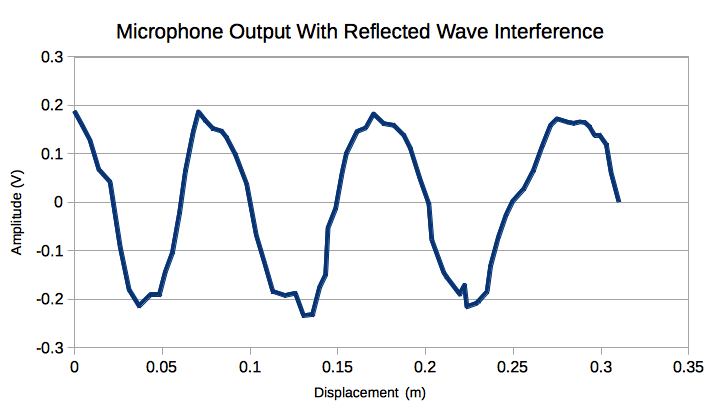
\includegraphics[width=80mm]{interference.png}
\caption{Graph of microphone measurements as a function of reflected wave
displacement relative to an arbitrary starting point. Measurements collected at
10 Hz.}
\label{fig:interference}
\end{figure}

\section{Analysis}

A linear regression of the dispersion relation in Figure~\ref{fig:dispersion},
taken through the origin, yields a slope of $357 \pm 14$ m/s. This regression
has an $r^2$ of 0.994, demonstrating that in the given range the ratio of the
angular frequency and wave number (the speed of sound) are very nearly
constant.

The amplitude variation in Figure~\ref{fig:interference} is not clear at every
point, so the region that appears to best fit a sine wave was used - from the
antinode at $0.098 \pm 0.003$ m to the antinode at $0.32 \pm 0.01$ m. This
corresponds to two full wavelengths, which with emitted sound frequency $3000
\pm 10$ Hz yields a speed of $333 \pm 14$.

\section{Conclusion}

The results of measuring the wavelength at varying frequencies shows a good
linear relation. The slope, corresponding to the speed of sound, was measured
to be $357 \pm 14$ m/s. This is different from the accepted value of 343.3 m/s
by 4\%, but it is within the uncertainty. The fit itself appears to be very
linear, with an $r^2$ of 0.994, showing that in the measured range (3 - 14 kHz)
the speed of sound is constant.

The speed of sound measured using interference antinodes was slightly closer,
at $333 \pm 14$. This is a difference of -3\% from the accepted value, and also
within the measurement uncertainty.

\end{document}


